%!TEX root = SysSpec_ClockPendulumAnalyzer.tex
\subsection{Umsetzung Sensor} %TODO describe schemantic 1 and 2 each
	Die Aufbau der Messvorrichtung des Sensors und dessen Anschluss ist nach folgenden Kriterien erfolgt:
	\begin{itemize}
		\item Flexible Positionierung des Sensors in der Höhe.
		\item Kleine Baugrösse um auch in kleineren Uhren messen zu können.
		\item Möglichst einfacher Anschluss mit Sicherung gegen Fehler.
	\end{itemize}
	Für den Betrieb des in Kapitel \ref{cap:sensoren} beschriebenen IR-Sensors sim im Datenblatt die in Abbildung \ref{fig:info_SFH9201} gegeben.
	\begin{figure}[H]
		\centering
		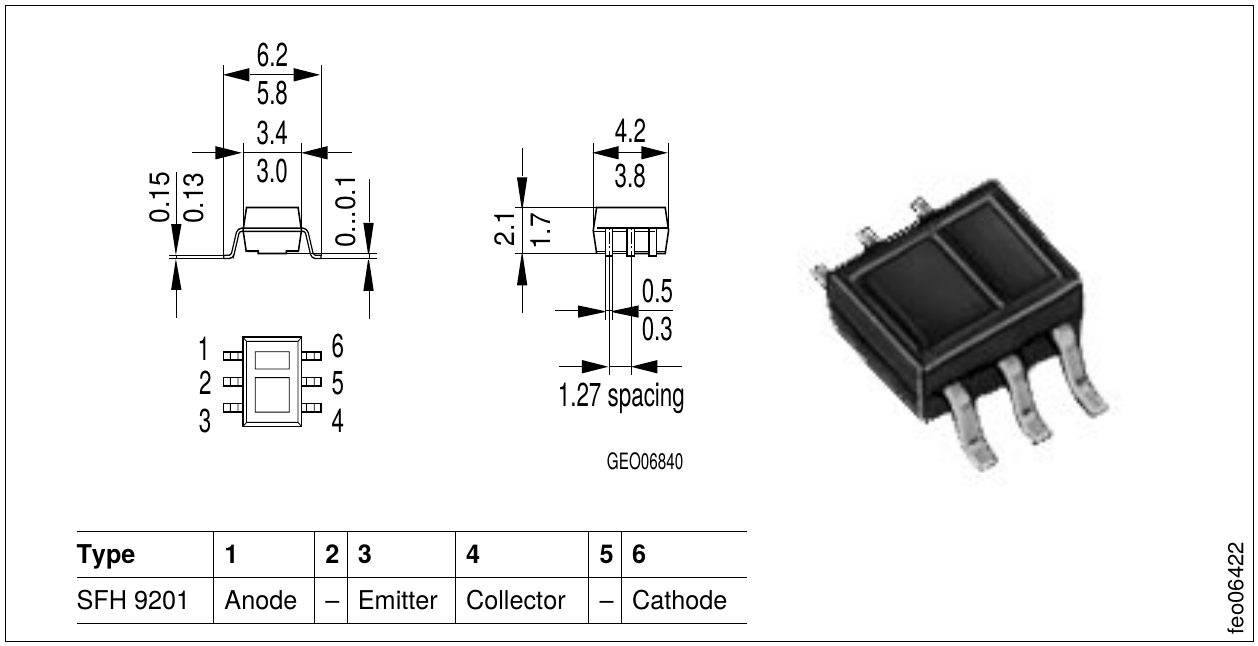
\includegraphics[width=.7\textwidth]{Sensor_layout}
		\caption{Anschlussinformationen SFH9201 (Bildquelle aus Datenblatt)}
		\label{fig:info_SFH9201}
	\end{figure}
	Da die Speisung der Diode und des Emitters in unserem Falle identisch sind, ist folgendes Schema daraus abgeleitet worden (Abbildung ).
	\begin{figure}[H]
		\centering
		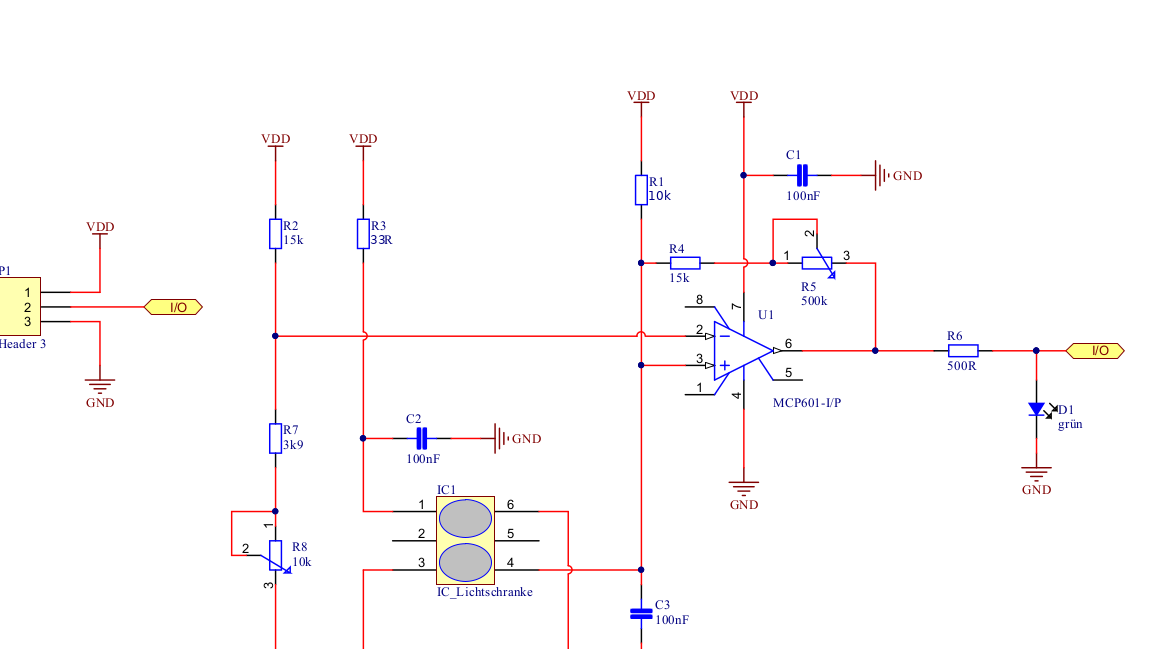
\includegraphics[width=.5\textwidth]{Circuit_Sensor}
		\caption{Ermitteltes Elektroschema für das Sensor-PCB SFH9201}
		\label{fig:schema_sensor}
	\end{figure}
	Die Diode vor dem Sensor verhindert ein falschs Anschliessen der IR-Diode und des Emitters. Der Widerstand von 24$\Omega$ ist der Vorgabe gemäss Datenblatt berechnet. Diese sind:
	\begin{itemize}
		\item 1.65V als maximale und gemessene Spannung $U_{IRD}$ über der IR-Diode
		\item 50mA Betriebsstrom $I_F$
	\end{itemize}
	Ausgehend von einer Speisung $U_S$ von 3.3V und einer Verlustspannung $U_V$ von 0.5V über der Sperrdiode ergibt dies folgende Formel:
	\[
		R = \frac{U_S - U_V - U_{IRD}}{I_R} = \frac{3.3 - 0.5 - 1.65}{0.05} = 23\Omega
	\]
	Ein entsprechendes PCP ist an der Hochschule Luzern, Technik \& Archtektur erstellt worden.\\
	Als Stütze für den Sensor dient eine Holzkonstruktion, welche über ein Lochraster von 10mm verfügt, an welchen sich der Sensor befestigen lässt. So können verschiedene Pendellängen und Anordungen angedeckt werden (Abbildung \ref{fig:Sensor_overview}).
	\begin{figure}[H]
		\centering
		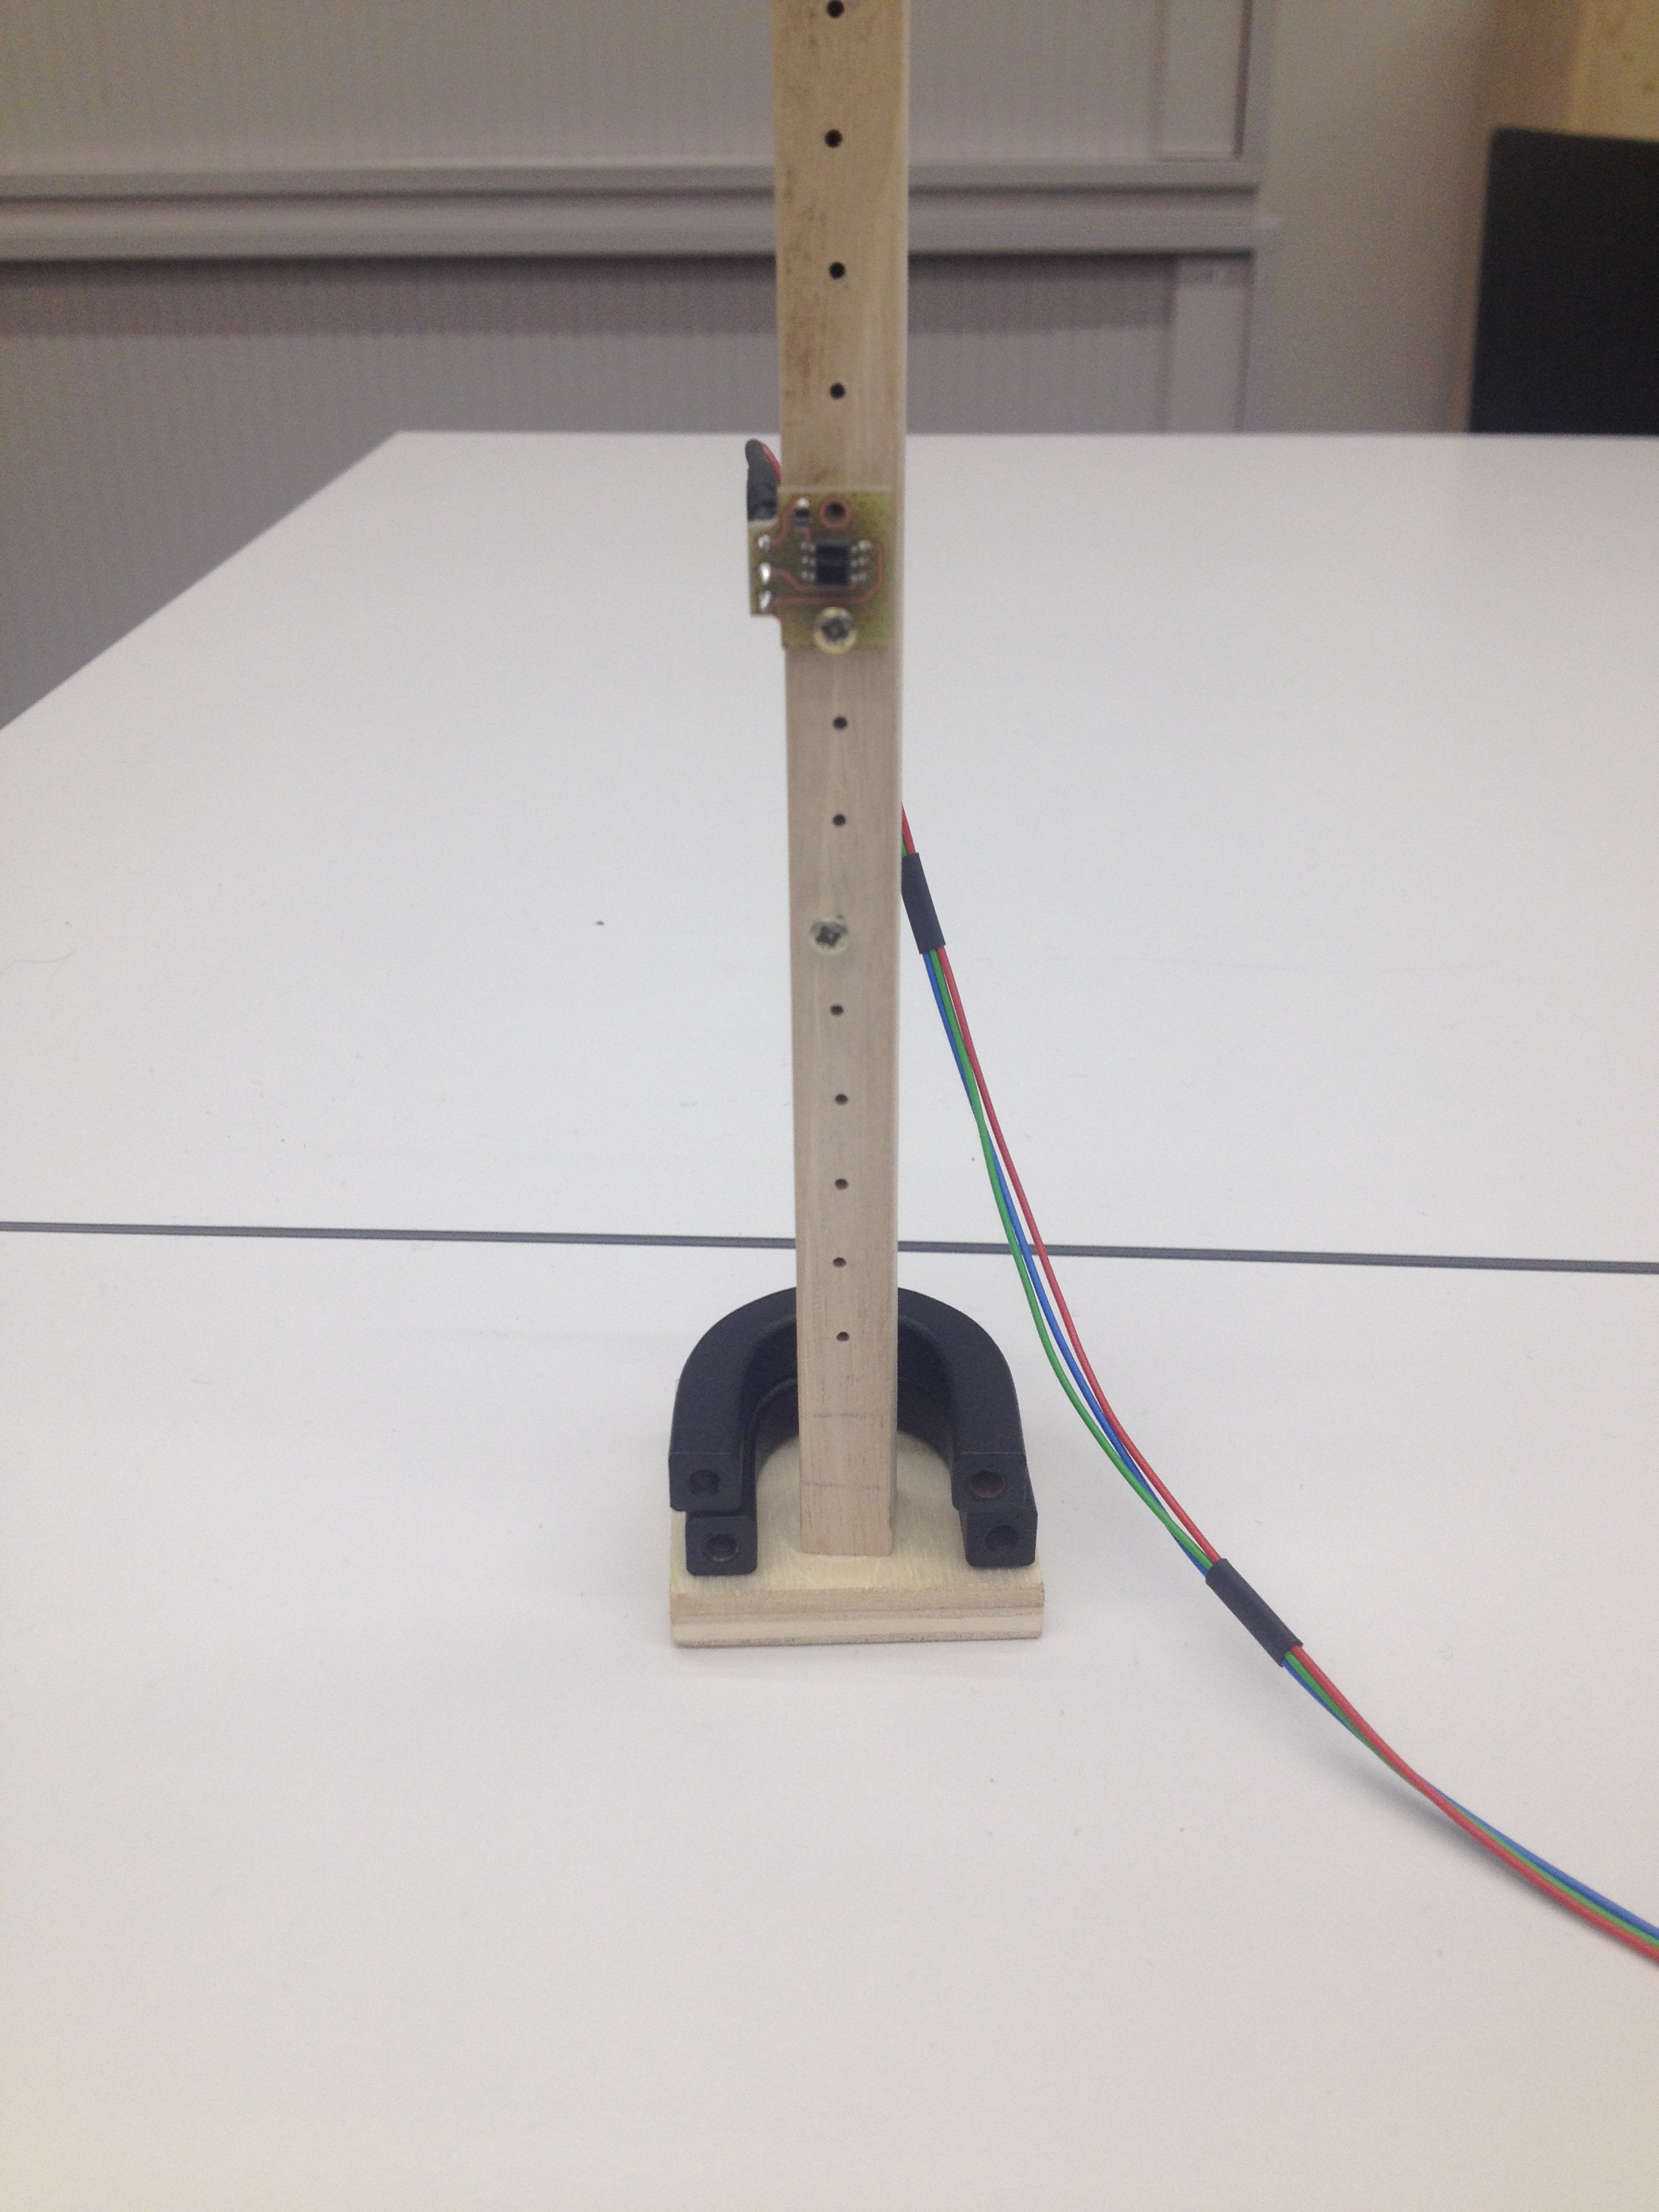
\includegraphics[width=.4\textwidth]{Sensor_overview}
		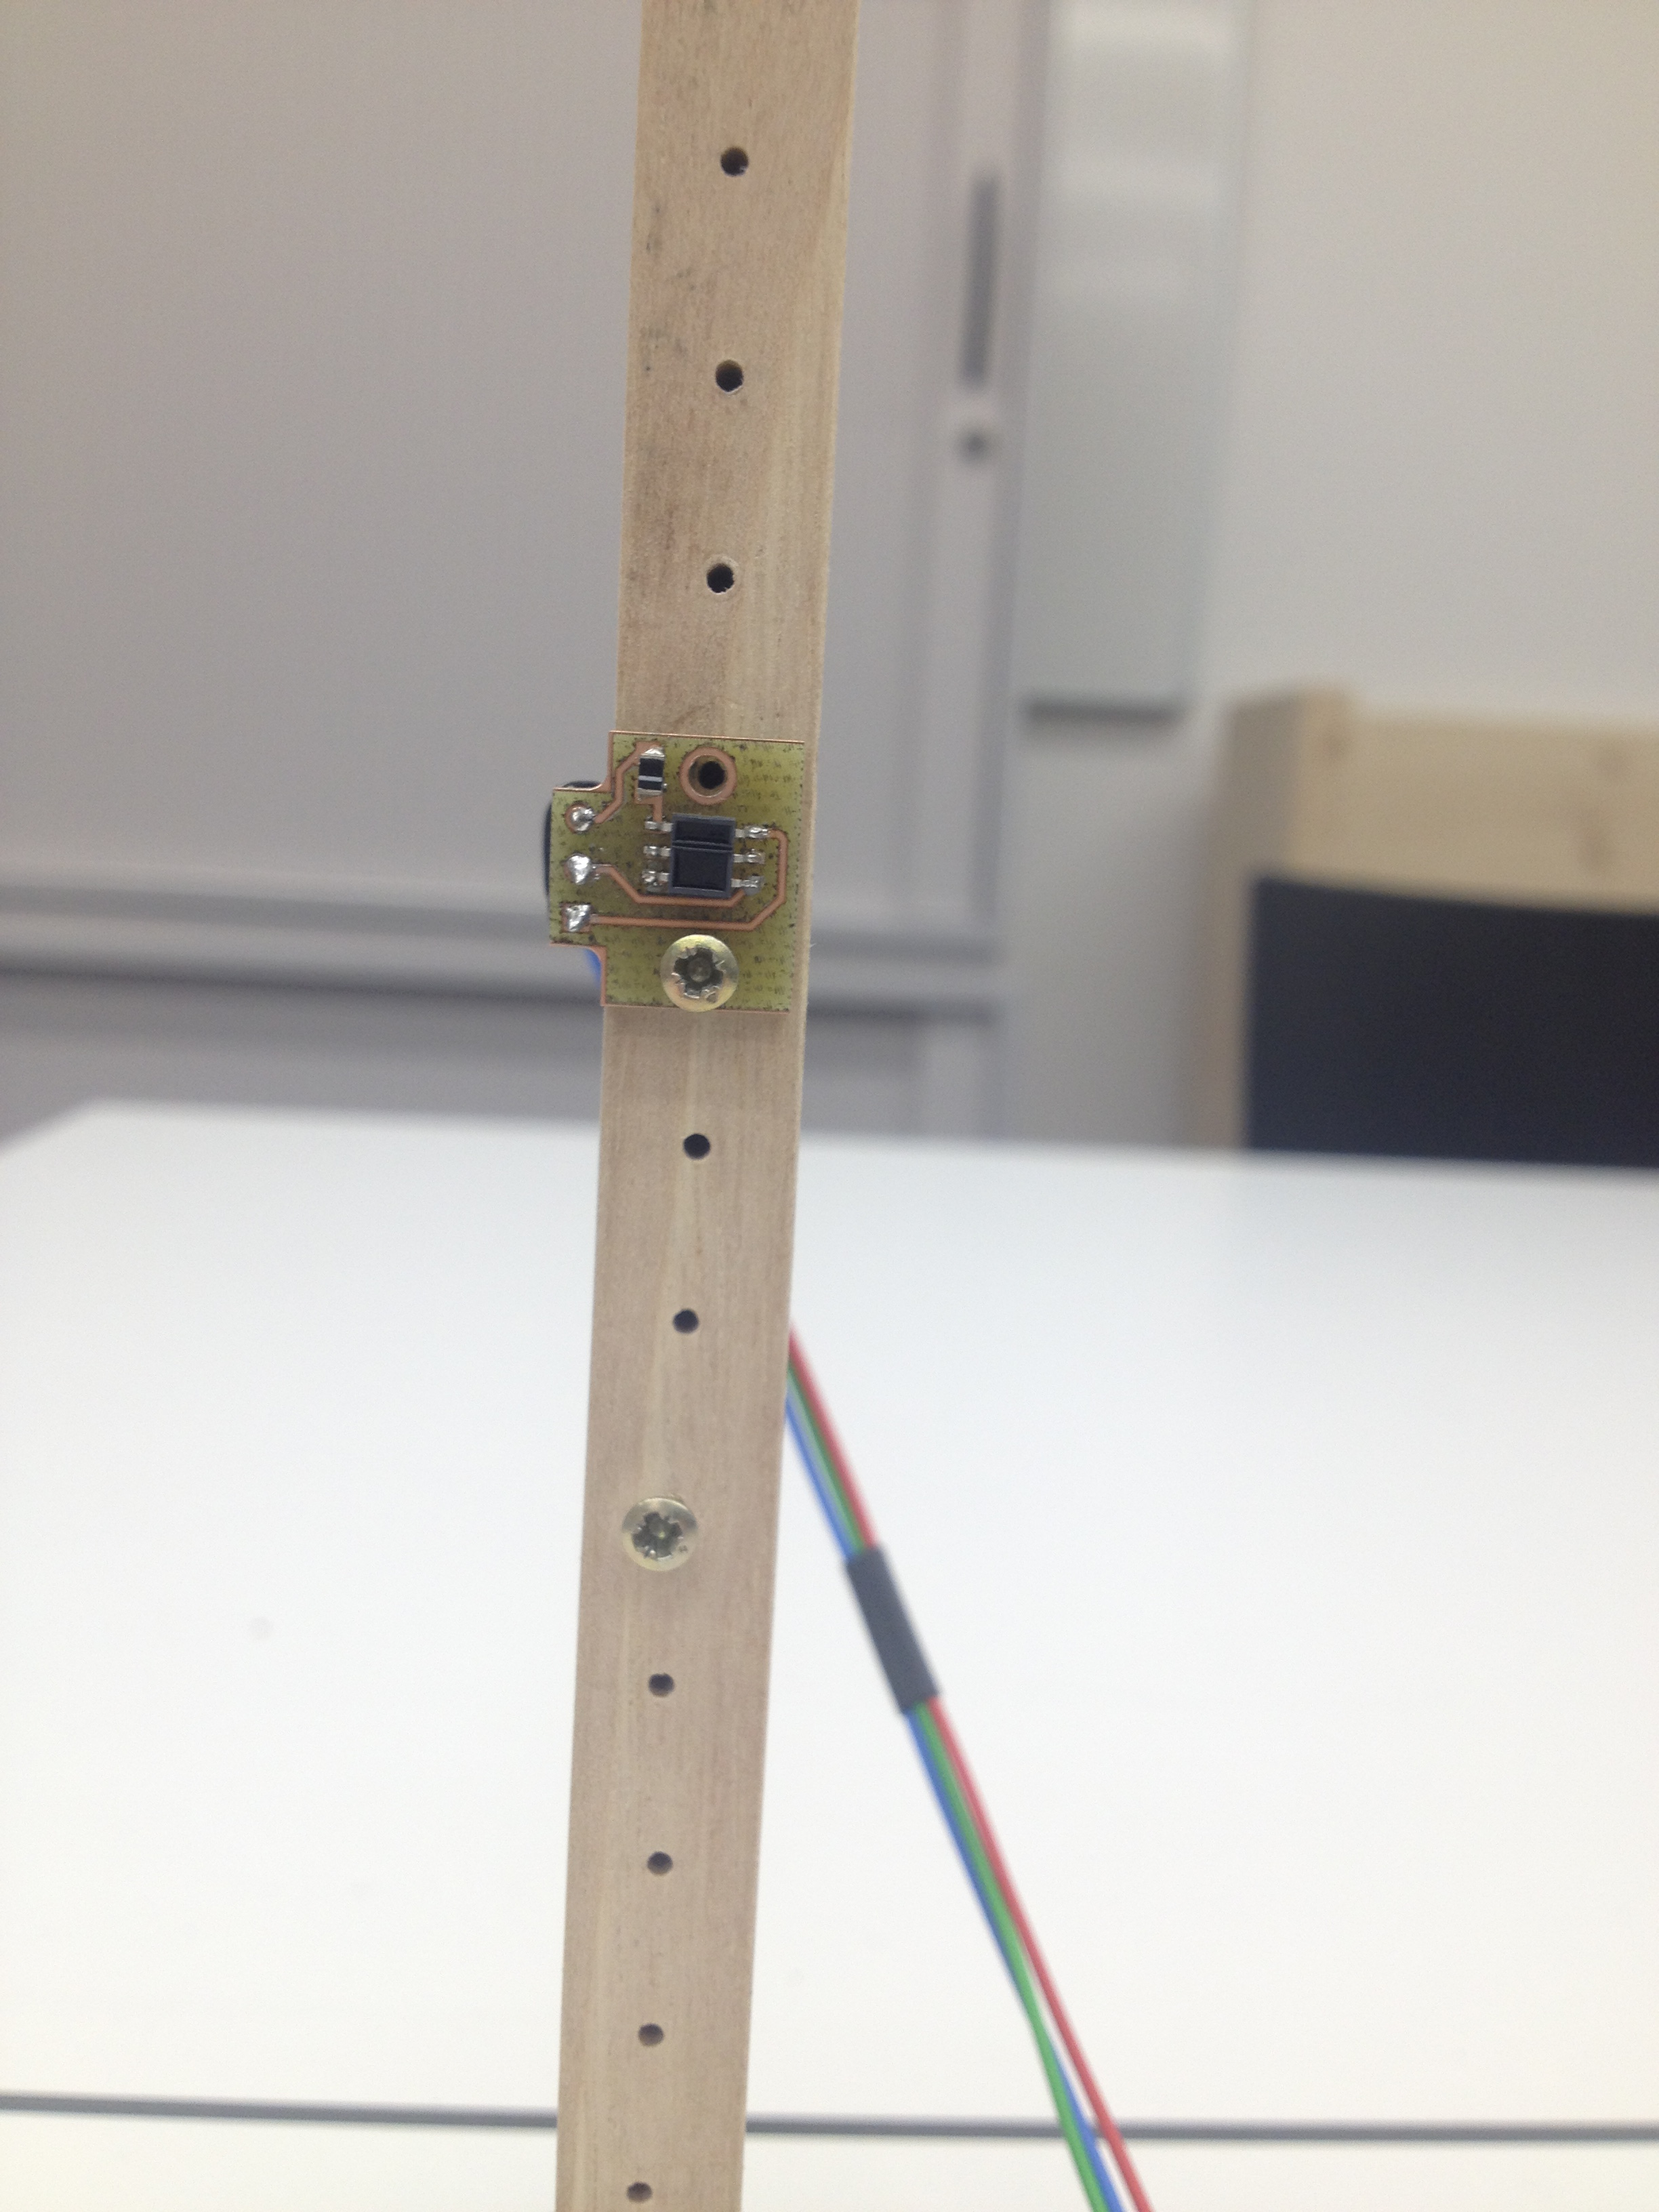
\includegraphics[width=.4\textwidth]{Sensor_Detail}
		\caption{Aufbau des Sensors für die Pendelmessung}
		\label{fig:Sensor_overview}
	\end{figure}